\section{Experiments}
\label{sec:experiments}

\subsection{Experimental Setup}
\label{sec:setup}

\paragraph{Models.}
Following prior work on multi-turn OPD~\citep{wang2026tcod}, we use teacher and student models from the same model family to reduce confounding effects from tokenizer, architecture, and instruction-format mismatch.
%
Specifically, we use Qwen3-32B and Qwen3-8B as teacher models, and Qwen3-0.6B and Qwen3-1.7B as student models~\citep{yang2025qwen3}. 
%
This yields multiple teacher--student pairs with different capacity gaps, allowing us to evaluate whether \ours remains effective across both large-gap and moderate-gap distillation settings.
%

\paragraph{Benchmarks and Evaluation Metrics.}
We evaluate \ours on three multi-turn agent benchmarks: ALFWorld~\citep{shridhar2020alfworld}, ScienceWorld~\citep{wang2022scienceworld}, and SearchQA~\citep{jin2025search}. 
%
These benchmarks cover embodied interaction, scientific task solving, and search-based question answering, respectively, allowing us to assess the effectiveness of selective intervention across different forms of multi-turn decision making.
%
For ALFWorld, we report success rate (SR) on both the seen and unseen splits. 
%
For ScienceWorld, we report success rate (SR) and the mean score on the test set. 
%
And for SearchQA, we report exact match (EM) across different question-answering datasets. 
%
Detailed definitions of the evaluation metrics are provided in \appref{sec:implementation_details}.
%


\paragraph{Baselines.}
We compare \ours with four main baselines: off-policy SFT, standard OPD~\citep{lu2025onpolicydistillation}, TCOD-F2B~\citep{wang2026tcod}, and Entropy-Aware OPD~\citep{jin2026entropy}. 
%
TCOD-F2B stabilizes multi-turn OPD through a forward-to-backward temporal curriculum, and Entropy-Aware OPD augments OPD with entropy-gated KL loss originally designed for single-turn distillation. 
%
Since \ours uses one additional teacher query to obtain the turn-level intervention label, we include an additional compute-matched baseline, OPD with two rollouts, where both the student and teacher are queried twice during OPD data collection without selective intervention. 
%
This controls for the additional teacher-query budget.
%

\paragraph{Training Details.}
We implement OPD with a fully asynchronous training pipeline. 
%
Unless otherwise specified, all methods are trained for one epoch with learning rate $1\times10^{-6}$ and rollout number 1. 
%
For \ours, we set the weak-intervention coefficient to $\alpha=0.5$. 
%
We analyze the sensitivity to this choice in \secref{sec:sensitivity_analysis}. 
%
Additional implementation details are provided in \appref{sec:implementation_details}.
%


\subsection{Main Results}
\label{sec:result_analysis}
%
\begin{table*}[t]
\centering
\caption{
    Main results on ALFWorld. 
    %
    We report success rate (SR) and average number of turns on both seen and unseen splits. 
    %
    Best and second-best SR among distillation methods for each setup is in \textbf{bold} and \underline{underlined}, respectively.
}
\vspace{-0.1in}
\label{tab:main_results_alfworld}
\setlength{\tabcolsep}{14pt}
\resizebox{\textwidth}{!}{%
\begin{tabular}{lllcccc}
\toprule
\textbf{Student Model} & \textbf{Teacher Model} & \textbf{Method}
& \textbf{Seen SR $\uparrow$} & \textbf{Seen Turns $\downarrow$}
& \textbf{Unseen SR $\uparrow$} & \textbf{Unseen Turns $\downarrow$} \\
\midrule
\multicolumn{7}{c}{\textit{Reference Models (Base Inference)}} \\
\midrule
Qwen3-0.6B & -- & Base & 1.43 & 29.65 & 0.75 & 29.82 \\
Qwen3-1.7B & -- & Base & 25.71 & 24.63 & 26.12 & 24.72 \\
-- & Qwen3-8B & Base & 61.43 & 17.95 & 67.16 & 17.24 \\
-- & Qwen3-32B & Base & 57.14 & 18.94 & 69.40 & 18.21 \\
\midrule
\multicolumn{7}{c}{\textit{Student: Qwen3-0.6B, Teacher: Qwen3-8B}} \\
\midrule
\multirow{6}{*}{Qwen3-0.6B} & \multirow{6}{*}{Qwen3-8B} & SFT & 2.86 & 29.32 & 4.48 & 28.87 \\
 & & OPD & 55.00 & 18.53 & 56.72 & 20.30 \\
 & & OPD (rollout 2) & \underline{56.43} & 18.76 & 59.70 & 20.31 \\
 & & Entropy-Aware OPD & 54.26 & 18.12 & 54.48 & 20.75 \\
 & & TCOD-F2B & \underline{56.43} & 18.51 & \underline{61.19} & 18.82 \\
 & & \ours{} & \textbf{57.86} & 18.46 & \textbf{61.94} & 18.89 \\
\midrule
\multicolumn{7}{c}{\textit{Student: Qwen3-1.7B, Teacher: Qwen3-8B}} \\
\midrule
\multirow{6}{*}{Qwen3-1.7B} & \multirow{6}{*}{Qwen3-8B} & SFT & 25.00 & 24.58 & 26.12 & 24.54 \\
 & & OPD & 60.00 & 17.80 & 61.94 & 17.67 \\
 & & OPD (rollout 2) & 63.00 & 17.51 & 64.93 & 17.87 \\
 & & Entropy-Aware OPD & 63.57 & 17.28 & \underline{65.67} & 18.20 \\
 & & TCOD-F2B & \textbf{64.29} & 17.65 & 58.21 & 19.16 \\
 & & \ours{} & \textbf{64.29} & 18.14 & \textbf{70.15} & 17.86 \\
\midrule
\multicolumn{7}{c}{\textit{Student: Qwen3-0.6B, Teacher: Qwen3-32B}} \\
\midrule
\multirow{5}{*}{Qwen3-0.6B} & \multirow{5}{*}{Qwen3-32B} & OPD & 53.57 & 19.49 & 68.66 & 18.65 \\
 & & OPD (rollout 2) & 52.14 & 20.28 & \underline{70.37} & 18.21 \\
 & & Entropy-Aware OPD & 48.57 & 20.87 & 68.13 & 18.28 \\
 & & TCOD-F2B & \textbf{54.29} & 20.18 & 67.91 & 19.26 \\
 & & \ours{} & \textbf{54.29} & 19.85 & \textbf{70.90} & 17.98 \\
\midrule
\multicolumn{7}{c}{\textit{Student: Qwen3-1.7B, Teacher: Qwen3-32B}} \\
\midrule
\multirow{5}{*}{Qwen3-1.7B} & \multirow{5}{*}{Qwen3-32B} & OPD & 58.57 & 18.89 & \underline{74.85} & 17.16 \\
 & & OPD (rollout 2) & \underline{62.14} & 18.17 & 72.39 & 18.37 \\
 & & Entropy-Aware OPD & 60.00 & 18.80 & \textbf{79.10} & 16.75 \\
 & & TCOD-F2B & 57.14 & 19.42 & 73.13 & 17.87 \\
 & & \ours{} & \textbf{62.82} & 18.75 & 73.88 & 17.57 \\
\bottomrule
\end{tabular}%
}
\end{table*}
%
\begin{table*}[t]
\centering
\caption{
    Main results on ScienceWorld. 
    %
    We report success rate (SR), mean task score, and average number of turns. 
    %
    Best and second-best SR among distillation methods for each setup is in \textbf{bold} and \underline{underlined}, respectively.
}
\vspace{-0.1in}
\label{tab:main_results_scienceworld}
% \resizebox{0.9\textwidth}{!}{%
\setlength{\tabcolsep}{22pt}
\resizebox{\textwidth}{!}{%
\begin{tabular}{lllccc}
\toprule
\textbf{Student Model} & \textbf{Teacher Model} & \textbf{Method}
& \textbf{SR $\uparrow$} & \textbf{Mean Score $\uparrow$} & \textbf{Turns $\downarrow$} \\
\midrule
\multicolumn{6}{c}{\textit{Reference Models (Base Inference)}} \\
\midrule
Qwen3-0.6B & -- & Base & 3.36 & -43.51 & 21.38 \\
Qwen3-1.7B & -- & Base & 3.36 & -24.00 & 21.38 \\
-- & Qwen3-8B & Base & 10.74 & -16.09 & 21.67 \\
-- & Qwen3-32B & Base & 15.44 & -17.92 & 18.67 \\
\midrule
\multicolumn{6}{c}{\textit{Student: Qwen3-0.6B, Teacher: Qwen3-8B}} \\
\midrule
\multirow{5}{*}{Qwen3-0.6B} & \multirow{5}{*}{Qwen3-8B} & SFT & 2.01 & -31.84 & 23.94 \\
 & & OPD & 2.01 & -12.88 & 23.94 \\
 & & Entropy-Aware OPD & \textbf{3.36} & -11.52 & 23.44 \\
 & & TCOD-F2B & \underline{3.03} & -2.07 & 24.88 \\
 & & \ours{} & 2.01 & \textbf{+3.89} & 26.94 \\
\midrule
\multicolumn{6}{c}{\textit{Student: Qwen3-1.7B, Teacher: Qwen3-8B}} \\
\midrule
\multirow{5}{*}{Qwen3-1.7B} & \multirow{5}{*}{Qwen3-8B} & SFT & 2.01 & -17.56 & 23.28 \\
 & & OPD & 4.70 & -2.78 & 25.12 \\
 & & Entropy-Aware OPD & 3.36 & -3.13 & 25.91 \\
 & & TCOD-F2B & 4.70 & -9.68 & 24.06 \\
 & & \ours{} & \textbf{6.71} & \textbf{+0.24} & 25.30 \\
\midrule
\multicolumn{6}{c}{\textit{Student: Qwen3-0.6B, Teacher: Qwen3-32B}} \\
\midrule
\multirow{5}{*}{Qwen3-0.6B} & \multirow{5}{*}{Qwen3-32B} & SFT & 2.01 & -34.59 & 18.10 \\
 & & OPD & 3.36 & -28.46 & 20.79 \\
 & & Entropy-Aware OPD & 6.04 & -26.10 & 20.00 \\
 & & TCOD-F2B & 2.68 & -33.42 & 23.20 \\
 & & \ours{} & \textbf{6.04} & \textbf{-26.10} & 20.00 \\
\midrule
\multicolumn{6}{c}{\textit{Student: Qwen3-1.7B, Teacher: Qwen3-32B}} \\
\midrule
\multirow{5}{*}{Qwen3-1.7B} & \multirow{5}{*}{Qwen3-32B} & SFT & 2.01 & -15.61 & 23.23 \\
 & & OPD & 4.03 & -29.89 & 19.64 \\
 & & Entropy-Aware OPD & 3.36 & -14.99 & 23.59 \\
 & & TCOD-F2B & \underline{6.04} & \textbf{-14.89} & 22.02 \\
 & & \ours{} & \textbf{7.38} & -16.01 & 20.91 \\
\bottomrule
\end{tabular}%
}
\end{table*}
%
\begin{table*}[htbp]
\centering
\caption{
    Main results on SearchQA. 
    %
    We report exact match (EM) across seven question-answering datasets and their average. 
    %
    Best and second-best SR among distillation methods for each setup is in \textbf{bold} and \underline{underlined}, respectively.
}
\vspace{-0.1in}
\label{tab:main_results_searchqa}
\setlength{\tabcolsep}{4pt}
\resizebox{\textwidth}{!}{%
\begin{tabular}{lllcccccccc}
\toprule
\textbf{Student Model} & \textbf{Teacher Model} & \textbf{Method}
& \textbf{NQ $\uparrow$} & \textbf{TriviaQA $\uparrow$} & \textbf{PopQA $\uparrow$} & \textbf{HotpotQA $\uparrow$}
& \textbf{2WikiMQA $\uparrow$} & \textbf{Musique $\uparrow$} & \textbf{Bamboogle $\uparrow$} & \textbf{Avg. $\uparrow$} \\
\midrule
\multicolumn{11}{c}{\textit{Reference Models (Base Inference)}} \\
\midrule
Qwen3-0.6B & -- & Base & 5.60 & 15.40 & 0.40 & 6.00 & 8.40 & 1.20 & 3.20 & 5.74 \\
Qwen3-1.7B & -- & Base & 24.20 & 36.40 & 5.20 & 19.00 & 14.20 & 10.80 & 18.40 & 18.31 \\
-- & Qwen3-8B & Base & 34.60 & 53.00 & 14.00 & 38.20 & 37.40 & 28.80 & 45.60 & 35.94 \\
-- & Qwen3-14B & Base & 35.00 & 55.80 & 15.60 & 41.20 & 43.00 & 30.00 & 49.60 & 38.60 \\
\midrule
\multicolumn{11}{c}{\textit{Student: Qwen3-0.6B, Teacher: Qwen3-8B}} \\
\midrule
\multirow{5}{*}{Qwen3-0.6B} & \multirow{5}{*}{Qwen3-8B} & SFT & 14.40 & 23.60 & 5.80 & 13.20 & 11.69 & 2.23 & 6.40 & 11.05 \\
 & & OPD & 25.00 & 41.40 & 17.80 & 28.20 & 24.80 & 17.00 & 24.00 & 25.46 \\
 & & Entropy-Aware OPD & \textbf{25.60} & 40.00 & \textbf{18.80} & 28.80 & \textbf{25.60} & \underline{17.40} & \textbf{24.40} & \textbf{25.80} \\
 & & TCOD-F2B & \underline{25.40} & 41.00 & 15.60 & \underline{29.00} & 24.60 & 16.80 & 23.20 & 25.09 \\
 & & \ours{} & 25.20 & \textbf{41.60} & \underline{18.40} & \textbf{29.80} & 23.20 & 15.00 & \underline{24.00} & \underline{25.31} \\
\midrule
\multicolumn{11}{c}{\textit{Student: Qwen3-1.7B, Teacher: Qwen3-8B}} \\
\midrule
\multirow{5}{*}{Qwen3-1.7B} & \multirow{5}{*}{Qwen3-8B} & SFT & 27.40 & 39.60 & 11.60 & 21.20 & 8.80 & 12.00 & 20.00 & 20.09 \\
 & & OPD & 30.60 & 47.20 & 12.40 & 33.20 & 29.60 & \textbf{24.80} & 32.80 & 30.09 \\
 & & Entropy-Aware OPD & 29.40 & \underline{48.20} & 12.60 & 33.20 & \underline{30.20} & 23.80 & \textbf{36.80} & \underline{30.60} \\
 & & TCOD-F2B & \textbf{31.20} & 47.60 & 12.40 & \textbf{33.80} & 28.60 & 24.00 & \underline{36.00} & 30.51 \\
 & & \ours{} & \underline{30.00} & \textbf{48.40} & \textbf{12.80} & 33.20 & \textbf{30.40} & \underline{24.60} & \underline{36.00} & \textbf{30.77} \\
\bottomrule
\end{tabular}%
}
\end{table*}
%
We present the main results on ALFWorld, ScienceWorld, and SearchQA in \tabref{tab:main_results_alfworld}, \ref{tab:main_results_scienceworld}, and \ref{tab:main_results_searchqa}, respectively.
%
Across all three benchmarks, \ours substantially improves over base student models and off-policy SFT. 
%
On ALFWorld, Qwen3-0.6B improves massively from $1.43/0.75$ (seen/unseen splits) SR to $57.86/61.94$ with a Qwen3-8B teacher, while reducing the average number of turns from nearly 30 to under 20. 
%
Compared with standard OPD, \ours further improves Qwen3-0.6B from $55.00$ to $57.86$ seen SR and from $56.72$ to $61.94$ unseen SR, while improving Qwen3-1.7B unseen SR from $61.94$ to $70.15$. 
%
Notably, these gains are not merely due to extra teacher queries, as \ours also outperforms the compute-matched OPD rollout-$2$ baseline in most ALFWorld settings, with comparable or fewer turns on the unseen split.
%


% \paragraph{Comparison with Strong OPD Variants.}
Compared with TCOD-F2B and Entropy-Aware OPD, \ours is strongest on ALFWorld and remains competitive on ScienceWorld and SearchQA. 
%
On ALFWorld, \ours achieves the best unseen SR in three out of four student--teacher settings and ties for the best seen SR in two settings, while generally maintaining similar turn efficiency to the strongest baselines. 
%
On SearchQA, \ours obtains the best average EM for Qwen3-1.7B distilled from Qwen3-8B, improving over OPD from $30.09$ to $30.77$. 
%
On ScienceWorld, \ours achieves the best SR for Qwen3-1.7B with both Qwen3-8B and Qwen3-32B teachers, and improves the Qwen3-0.6B mean score with Qwen3-8B from $-12.88$ under OPD to $+3.89$, although this comes with a higher average number of turns, suggesting more sustained task exploration.
%

\paragraph{Effects of Student and Teacher Scale.}
We notice that the benefits of \ours are more consistent for the larger Qwen3-1.7B student, which achieves strong gains on ALFWorld, the best average SearchQA result, and the best ScienceWorld SR across both teacher settings. 
%
For Qwen3-0.6B, OPD already provides large gains over SFT and base inference, while \ours further improves ALFWorld generalization but shows more task-dependent effects on ScienceWorld and SearchQA. 
%
We also observe that merely increasing teacher size is not uniformly beneficial, we hypothesize that stronger teacher signals may not be always more reliable when applied densely and that adaptive weighting is important for multi-turn OPD.
%


\begin{figure*}[t]
    \centering
    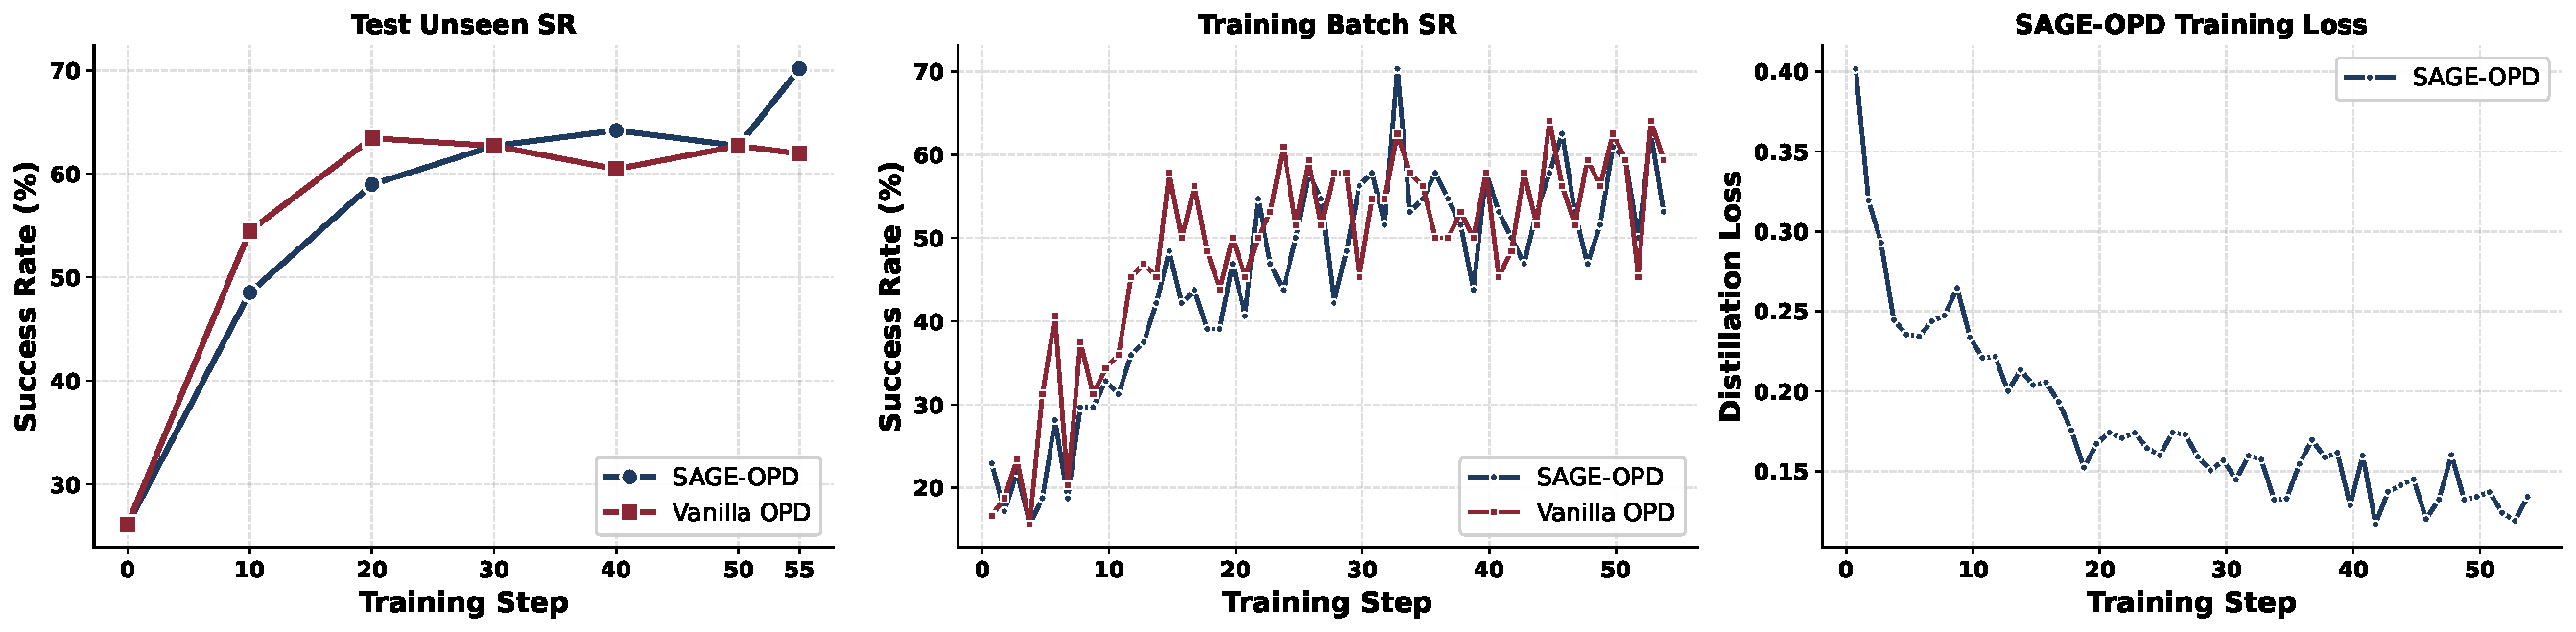
\includegraphics[width=\textwidth]{figure/alfworld_sl_opd_vs_vanilla.pdf}
    \caption{Training dynamics on ALFWorld comparing \ours{} with vanilla OPD. Left: test unseen success rate during training. Middle: training-batch success rate. Right: training loss of \ours{}.}
    \label{fig:training_dynamics}
\end{figure*}

\subsection{Training Dynamics}

\figref{fig:training_dynamics} compares the training dynamics of \ours and standard OPD~\citep{lu2025onpolicydistillation} on ALFWorld~\citep{shridhar2020alfworld}. 
%
On the unseen test split (\figref{fig:training_dynamics}-\textit{left}), both methods improve rapidly in the early stage, but standard OPD saturates after roughly 20--30 training steps and fluctuates around $60$--$63\%$ success rate. 
%
In contrast, \ours continues to improve in the later stage and reaches $70.15\%$ unseen success rate by the end of training. 
%
This suggests that selective intervention does not merely accelerate early learning, but also helps maintain useful teacher supervision after standard dense OPD begins to plateau.
%

% The training-batch success rate (\figref{fig:training_dynamics}-\textit{middle}) shows a similar trend: both methods improve throughout training, while \ours remains competitive with standard OPD despite applying supervision selectively rather than uniformly.
The training-batch success rate (\figref{fig:training_dynamics}-\textit{middle}) shows the two methods tracking each other closely throughout training, so selective supervision fits the on-policy training distribution about as well as dense OPD while intervening on only a subset of turns.
%
This contrast (comparable training-batch success but a widening gap on the unseen split) shows that selective intervention improves generalization rather than training-distribution fit.
%
\figref{fig:training_dynamics}-\textit{right} further shows that the \ours distillation loss decreases steadily over training, indicating stable optimization under the intervention-weighted objective. 
%
Together, these dynamics support our hypothesis that selectively reallocating teacher supervision can improve generalization while preserving stable on-policy training.